
\paragraph*{Potential Issues}
\label{sec:findings-r2-potentialissues}

%%%
The comparable performance to random weights must be addressed as a potential
error in implementation rather than in training.
%
Since all methods of training so far have resulted in very similar policies
being learned,
it is fair to say that policy learned during training has been superior to
random in some manner.
%
There are then a few items to consider with regard to why such poor results are occurring
during the review tournaments.
%%%


\subparagraph*{Overfitting}

%%%
% Overfitting
The first item to consider as the source of the discrepancy between the
observation that a policy is learned,
but its performance is abysmal
is that the weights table is overfitting to the problem.
%
This would have been especially true of the first round where learning rates
were much higher.
%
However,
if the agents were to be overfitting,
a number of differences would be found in their results.
%
Firstly,
a different set of policy graphs would likely result from the training phase
which is not the case.
%
More importantly,
a definitive curve would be present in the tournament graphs as performance
would increase before dropping.
%
As can be seen in Figures~\ref{fig:r2-spreads-winner}
and~\ref{fig:r2-spreads-loser},
this is not the case
as performance is not apparently linked to training in any way.
%
Therefore, it would seem safe to conclude that overfitting is not the reason
for the poor resulting performance.
%%%


\subparagraph*{Scale of Play}

%%%
The prevailing theory as to the reason for which the agent learns a policy,
but following that policy does not yield positive results in performance,
is the issue of scale.
%
The agent is trained on a million games,
but tested on only a handful.
%
Since the cards being dealt are not taken into account by the policy,
the decisions made will likely be inaccurate on the scale of a single game,
but not for thousands.
%%%

% Figures

\begin{figure}
\center
\begin{subfigure}[b]{0.45\textwidth}
	\center
	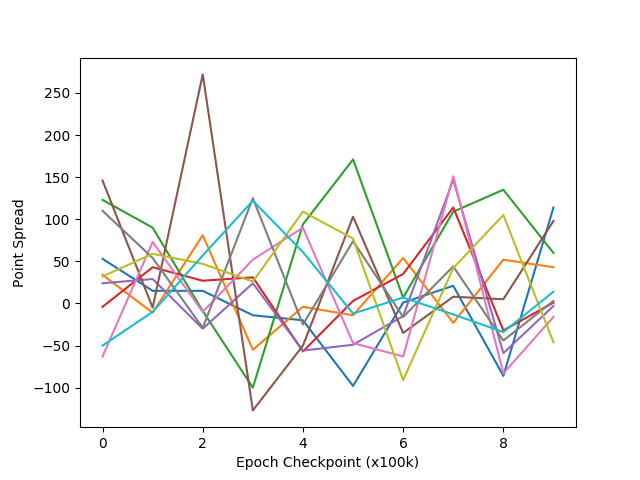
\includegraphics[width=\textwidth]{images/discussion/usefulness/r2-time-series-9.png}
	\caption{Point spreads for 9-game matches} %, like in human play.}
	\label{fig:r2-time-series-9}
\end{subfigure}
~
\begin{subfigure}[b]{0.45\textwidth}
	\center
	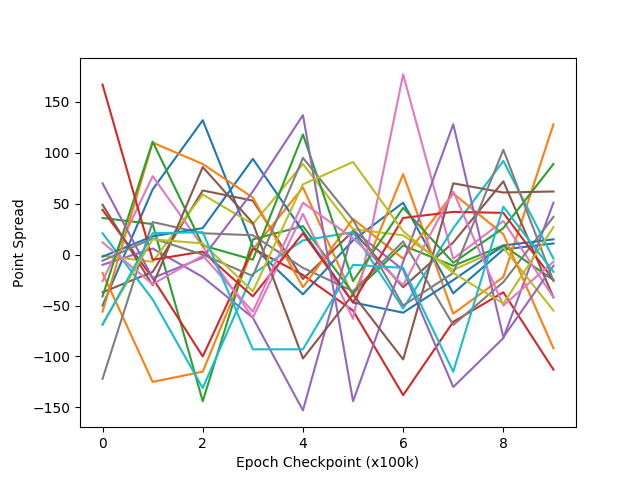
\includegraphics[width=\textwidth]{images/discussion/usefulness/r2-time-series-100.png}
	\caption{Point spreads for 100-game matches.}
	\label{fig:r2-time-series-100}
\end{subfigure}

\begin{subfigure}[b]{0.66\textwidth}
	\center
	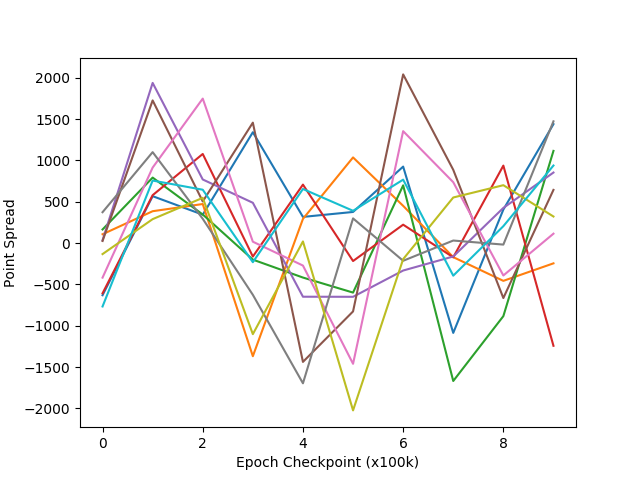
\includegraphics[width=\textwidth]{images/discussion/usefulness/r2-time-series-1000.png}
	\caption{Point spreads for 1,000-game matches.}
	\label{fig:r2-time-series-1000}
\end{subfigure}

\begin{subfigure}[b]{0.66\textwidth}
	\center
	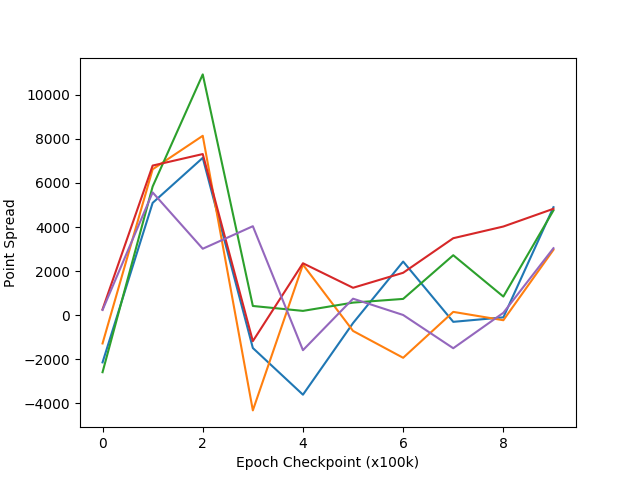
\includegraphics[width=\textwidth]{images/discussion/usefulness/r2-time-series-10000.png}
	\caption{Point spreads for 10,000-game matches.}
	\label{fig:r2-time-series-10000}
\end{subfigure}

\caption{
	Point spreads across matches of varying lengths.
	In each graph,
	the final trained agent is played against its previous checkpoint
	iterations.
}
\label{fig:r2-time-series}
\end{figure}

% /Figures

%%%
% Discussion of how scale affects score spreads
%	On 9-game scale, we have utter chaos, maybe not worth mentioning?
%	On 100-game scale, utter chaos
%	On 1000-game scale, maybe a little, if we squint hard,
%	On 10k-game scale, we can see a pattern
%		contradicts the 1k-game observations
%		consistently even with random
%		sharp increase in performance over 100k-200k
%		even play for the next 600k
%		seemingly regain advantage in the last 200k
%%%

%%%
A regulation cribbage match between two human players consists of nine games.
%
As can be seen in Figure~\ref{fig:r2-time-series-100},
in a series of 100-game matches between a fully trained agent and its
previous checkpoints\textemdash
using a Round 2-trained agent in the loser's bracket for demonstrative
purposes\textemdash
no pattern is discernible in total point spreads between the two playing agents.
%
This demonstrates that,
on this scale,
the winner of the game is no more predictable than a truly random coin toss.
%%%

%%%
When the scale is increased to one thousand games,
a slight pattern begins to emerge
when visualized in Figure~\ref{fig:r2-time-series-1000}.
%
Whereas the majority of the graph remains highly varying and unpatterned,
the first few games follow a common pattern.
%
The match against the random agent is still unpredictable,
but the matches against the 100,000 and 200,000 game trained checkpoints are
consistently beaten by the final agent.
%%%

%%%
Although fewer matches are played to compensate for the increased time needed to
play the increased number of games,
the same pattern present in the thousand-game scale is visible in the
ten thousand-game matches.
%
With the exception of the purely untrained agent,
the least \learned\ agents perform the poorest against the final
\learned\ agent.
%
Play is approximately evenly matched between the fully trained agent
and its checkpoints which have been trained for 300,000 to 700,000 games.
%
Following these matches,
the agent begins to, again, win more consistently when more training is done.
%
This confusingly indicates that more recent agents are getting worse
than earlier iterations,
but that the final agent is better than these.
%%%

%%%
If the agent is being trained correctly and no overfitting is occurring,
then the point spread should be a positive number,
gradually decreasing and approaching zero
as more training is applied to its opponent,
forming a similar curve to a loss metric used in classical machine learning.
%
In the event of overfitting,
the curve would dip below the zero before reapproaching zero.
%
Neither of these shapes were seen in the resulting graph
(see Figure~\ref{fig:r2-time-series-10000}).
%
Instead,
the shape of the curve implies that,
since the random agent performs consistently better than the trained agent,
the learning process is not learning the game so much as how to outplay its
opponent in some corner case that does not reappear during testing.
%
This conclusion is supported by the observation that the agents with limited
training are steadfastly outplayed.
%%%

%%%
However,
since there is a sharp dip after 300,000 training epochs before increasing
again,
the results are difficult to interpret.
%
The final \learned\ agent is more evenly matched in performance with an agent
trained for 400,000 games
than it is against a more recently trained agent.
%
The reintroduction of an increasing curve
is an indicator of overfitting in the middle stages.
%
Whereas the final agent is able to play well against these agents,
they themselves have decreased in performance capability.
%
This can be speculated to be a result of learning how to outplay its opposing agent
rather than an understanding of the game,
but similar performance when the opposing agent
has fixed random weights\textemdash
as can be seen in comparisons between Figures
\ref{fig:r2-spreads-winner} and \ref{fig:r2-spreads-random}\textemdash
counters this postulate.
%%%

%%%
Also of further note, is the scale on the aforementioned graphs.
%
In Figure~\ref{fig:r2-time-series-10000},
the maximum point spread achieved is just a shade above 10,000 points
over the course of 10,000 games.
%
This means that the average point spread advantage is approximately 
one point per game at peak performance\textemdash
and most often $0.2$ points per game\textemdash
in long-term play.
%
The average spread increases to $25$ points per game when fewer games are 
played,
but since performance is unpredictable on this scale,
this can be explained as a result of the randomness of the cards given
and cannot be considered a reliable measure of performance.
%
In fact,
in sampled matches,
it was not uncommon to observe losses and wins of 30 points or more
as well as much closer games with margins of only a few points.
%
In addition to the randomness of cards dealt,
this massive point sway could also be the result of the agents' uncertainty on 
how to recover from a losing position.
%
While the reasons for this inability cannot be said to be more than speculation,
the learning of a policy directly without taking into account cards dealt
is the likely culprit,
as explained previously.
%%%

